% interpolacion_bicubica_R_completo_tikz_final5.tex
% Versión final con fórmulas más a la izquierda y títulos separados

\begin{figure}[h]
\centering
\begin{tikzpicture}[
    font=\normalsize,
    cell/.style={rectangle, draw=black, minimum size=0.9cm, inner sep=0},
    legendcell/.style={rectangle, draw=black, minimum size=0.8cm, inner sep=0},
    formula/.style={font=\footnotesize, align=left}
]

% ============================================
% PARÁMETROS DE LA CUADRÍCULA
% ============================================
\def\gridWidth{16}   % Ancho total aumentado (en cm)
\def\rowOneHeight{3.5}  % Alto de la fila 1 (en cm)
\def\rowTwoHeight{5.0}  % Alto de la fila 2 reducido (en cm)
\def\colWidth{2.8}    % Ancho de cada columna (en cm)

% ============================================
% DEFINICIÓN DE COORDENADAS DE CENTRO
% ============================================
% Fila 1 (5 columnas)
\coordinate (F1C1) at (0.5*\colWidth, 0);
\coordinate (F1C2) at (1.5*\colWidth, 0);
\coordinate (F1C3) at (2.5*\colWidth, 0);
\coordinate (F1C4) at (3.5*\colWidth, 0);
\coordinate (F1C5) at (4.5*\colWidth, 0);

% Fila 2 (ocupa ancho completo)
\coordinate (F2) at (2.5*\colWidth, -\rowOneHeight-0.5*\rowTwoHeight);

% ============================================
% F1C1: MATRIZ ORIGINAL - CANAL R (4×4) CORREGIDA
% ============================================
\begin{scope}[shift={(F1C1)}]
    % Título
    \node[above, font=\bfseries, red!80!black] at (0, 2.2) {Canal R Original (4×4)};
    
    % Matriz 4x4 con valores en posiciones correctas según patrón Bayer
    % Fila 1 (índice 1)
    \node[cell, fill=red!80!black] at (-1.35, 1.35) {\textcolor{white}{$r_{11}$}};
    \node[cell, fill=gray!20] at (-0.45, 1.35) {$0$};
    \node[cell, fill=red!80!black] at (0.45, 1.35) {\textcolor{white}{$r_{13}$}};
    \node[cell, fill=gray!20] at (1.35, 1.35) {$0$};
    
    % Fila 2 (índice 2)
    \node[cell, fill=gray!20] at (-1.35, 0.45) {$0$};
    \node[cell, fill=gray!20] at (-0.45, 0.45) {$0$};
    \node[cell, fill=gray!20] at (0.45, 0.45) {$0$};
    \node[cell, fill=gray!20] at (1.35, 0.45) {$0$};
    
    % Fila 3 (índice 3)
    \node[cell, fill=red!80!black] at (-1.35, -0.45) {\textcolor{white}{$r_{31}$}};
    \node[cell, fill=gray!20] at (-0.45, -0.45) {$0$};
    \node[cell, fill=red!80!black] at (0.45, -0.45) {\textcolor{white}{$r_{33}$}};
    \node[cell, fill=gray!20] at (1.35, -0.45) {$0$};
    
    % Fila 4 (índice 4)
    \node[cell, fill=gray!20] at (-1.35, -1.35) {$0$};
    \node[cell, fill=gray!20] at (-0.45, -1.35) {$0$};
    \node[cell, fill=gray!20] at (0.45, -1.35) {$0$};
    \node[cell, fill=gray!20] at (1.35, -1.35) {$0$};
\end{scope}

% ============================================
% F1C2: FLECHA DE PROCESO
% ============================================
\begin{scope}[shift={(F1C2)}]
    \node[font=\Huge] at (0, 0) {$\Rightarrow$};
    \node[above, font=\scriptsize] at (0, 1) {Interpolación};
    \node[below, font=\scriptsize] at (0, -1) {Bicúbica};
\end{scope}

% ============================================
% F1C3: MATRIZ INTERPOLADA - CANAL R (4×4)
% ============================================
\begin{scope}[shift={(F1C3)}]
    % Título
    \node[above, font=\bfseries, red!80!black] at (0, 2.2) {Canal R Interpolado (4×4)};
    
    % Matriz 4x4 completa
    % Fila 1
    \node[cell, fill=red!80!black] at (-1.35, 1.35) {\textcolor{white}{$r_{11}$}};
    \node[cell, fill=red!70!black] at (-0.45, 1.35) {\textcolor{white}{$r_{12}$}};
    \node[cell, fill=red!80!black] at (0.45, 1.35) {\textcolor{white}{$r_{13}$}};
    \node[cell, fill=red!70!black] at (1.35, 1.35) {\textcolor{white}{$r_{14}$}};
    
    % Fila 2
    \node[cell, fill=red!70!black] at (-1.35, 0.45) {\textcolor{white}{$r_{21}$}};
    \node[cell, fill=red!50!black] at (-0.45, 0.45) {\textcolor{white}{$r_{22}$}};
    \node[cell, fill=red!60!black] at (0.45, 0.45) {\textcolor{white}{$r_{23}$}};
    \node[cell, fill=red!70!black] at (1.35, 0.45) {\textcolor{white}{$r_{24}$}};
    
    % Fila 3
    \node[cell, fill=red!80!black] at (-1.35, -0.45) {\textcolor{white}{$r_{31}$}};
    \node[cell, fill=red!60!black] at (-0.45, -0.45) {\textcolor{white}{$r_{32}$}};
    \node[cell, fill=red!80!black] at (0.45, -0.45) {\textcolor{white}{$r_{33}$}};
    \node[cell, fill=red!60!black] at (1.35, -0.45) {\textcolor{white}{$r_{34}$}};
    
    % Fila 4
    \node[cell, fill=red!70!black] at (-1.35, -1.35) {\textcolor{white}{$r_{41}$}};
    \node[cell, fill=red!50!black] at (-0.45, -1.35) {\textcolor{white}{$r_{42}$}};
    \node[cell, fill=red!60!black] at (0.45, -1.35) {\textcolor{white}{$r_{43}$}};
    \node[cell, fill=red!70!black] at (1.35, -1.35) {\textcolor{white}{$r_{44}$}};
\end{scope}

% ============================================
% F1C5: LEYENDA DE COLORES CORREGIDA
% ============================================
\begin{scope}[shift={(F1C5)}]
    % Título
    \node[above, font=\bfseries] at (0, 2.2) {Leyenda de Colores};
    
    % Ajuste vertical
    \def\verticalShift{0.6}
    
    % Original (rojo oscuro)
    \node[legendcell, fill=red!80!black] at (-1, 0.8+\verticalShift) {};
    \node[anchor=west, font=\small] at (-0.7, 0.8+\verticalShift) {Original};
    \node[anchor=west, font=\tiny] at (-0.7, 0.5+\verticalShift) {($r_{11}$, $r_{13}$, $r_{31}$, $r_{33}$)};
    
    % Interpolado 1D (rojo medio-alto)
    \node[legendcell, fill=red!70!black] at (-1, -0.1+\verticalShift) {};
    \node[anchor=west, font=\small] at (-0.7, -0.1+\verticalShift) {Interp. Borde};
    \node[anchor=west, font=\tiny] at (-0.7, -0.4+\verticalShift) {($r_{12}$, $r_{14}$, $r_{21}$, $r_{24}$)};
    
    % Interpolado 2D (rojo medio)
    \node[legendcell, fill=red!50!black] at (-1, -1.0+\verticalShift) {};
    \node[anchor=west, font=\small] at (-0.7, -1.0+\verticalShift) {Interp. 2D};
    \node[anchor=west, font=\tiny] at (-0.7, -1.3+\verticalShift) {($r_{22}$, $r_{23}$, $r_{32}$, $r_{34}$)};
    
    % Interpolado centro (rojo claro)
    \node[legendcell, fill=red!30!black] at (-1, -1.9+\verticalShift) {};
    \node[anchor=west, font=\small] at (-0.7, -1.9+\verticalShift) {Interp. Centro};
    \node[anchor=west, font=\tiny] at (-0.7, -2.2+\verticalShift) {($r_{42}$, $r_{43}$, $r_{44}$)};
    
    % Por interpolar (gris)
    \node[legendcell, fill=gray!20] at (-1, -2.8+\verticalShift) {};
    \node[anchor=west, font=\small] at (-0.7, -2.8+\verticalShift) {Por interpolar};
    \node[anchor=west, font=\tiny] at (-0.7, -3.1+\verticalShift) {(valor 0)};
\end{scope}

% ============================================
% F2: FÓRMULAS AÚN MÁS A LA IZQUIERDA CON TÍTULOS SEPARADOS
% ============================================
\begin{scope}[shift={(F2)}]
    % Título principal
    \node[above, font=\bfseries] at (0, 1.7) {Fórmulas de Interpolación Bicúbica};
    
    % Parámetros para espaciado uniforme - ajustados
    \def\titleSpacing{0.6}       % ESPACIO AUMENTADO después del título de sección
    \def\formulaSpacing{0.65}    % Espacio uniforme entre fórmulas
    \def\sectionSpacing{0.6}     % Espacio entre secciones
    \def\columnX{-6.5}           % COLUMNA MUCHO MÁS A LA IZQUIERDA
    
    % Coordenadas Y fijas - ajustadas
    \def\startY{1.5}
    \def\yOneTitle{\startY}
    \def\yOneA{\startY - \titleSpacing}        % Más espacio después del título
    \def\yOneB{\yOneA - \formulaSpacing}
    \def\yOneC{\yOneB - \formulaSpacing}
    \def\yOneD{\yOneC - \formulaSpacing}
    
    \def\yTwoTitle{\yOneD - \sectionSpacing}
    \def\yTwoA{\yTwoTitle - \titleSpacing}     % Más espacio después del título
    \def\yTwoB{\yTwoA - \formulaSpacing}
    \def\yTwoC{\yTwoB - \formulaSpacing}
    \def\yTwoD{\yTwoC - \formulaSpacing}
    
    % ========== INTERPOLACIONES 1D ==========
    % Subtítulo: Interpolación 1D - con más espacio debajo
    \node[anchor=west, font=\small\bfseries, align=left] at (\columnX, \yOneTitle) 
        {Interpolación 1D:};
    
    % Fórmulas 1D (alineadas a la izquierda)
    \node[anchor=west, formula, align=left] at (\columnX, \yOneA) 
        {$r_{12} = -\tfrac{1}{16}r_{10} + \tfrac{9}{16}r_{11} + \tfrac{9}{16}r_{13} - \tfrac{1}{16}r_{14}$};
    
    \node[anchor=west, formula, align=left] at (\columnX, \yOneB) 
        {$r_{14} = -\tfrac{1}{16}r_{12} + \tfrac{9}{16}r_{13} + \tfrac{9}{16}r_{15} - \tfrac{1}{16}r_{16}$};
    
    \node[anchor=west, formula, align=left] at (\columnX, \yOneC) 
        {$r_{21} = -\tfrac{1}{16}r_{01} + \tfrac{9}{16}r_{11} + \tfrac{9}{16}r_{31} - \tfrac{1}{16}r_{41}$};
    
    \node[anchor=west, formula, align=left] at (\columnX, \yOneD) 
        {$r_{41} = -\tfrac{1}{16}r_{21} + \tfrac{9}{16}r_{31} + \tfrac{9}{16}r_{51} - \tfrac{1}{16}r_{61}$};
    
    % ========== INTERPOLACIONES 2D ==========
    % Subtítulo: Interpolación 2D - con más espacio debajo
    \node[anchor=west, font=\small\bfseries, align=left] at (\columnX, \yTwoTitle) 
        {Interpolación 2D:};
    
    % Fórmulas 2D (alineadas a la izquierda)
    \node[anchor=west, formula, align=left, text width=14.5cm] at (\columnX, \yTwoA) 
        {$r_{22} = \tfrac{1}{256}(r_{00} - 9r_{01} - 9r_{10} + 81r_{11} + 81r_{13} - 9r_{14} - 9r_{30} + 81r_{31} + 81r_{33} - 9r_{34})$};
    
    \node[anchor=west, formula, align=left, text width=14.5cm] at (\columnX, \yTwoB) 
        {$r_{23} = \tfrac{1}{256}(r_{01} - 9r_{02} - 9r_{11} + 81r_{12} + 81r_{14} - 9r_{15} - 9r_{31} + 81r_{32} + 81r_{34} - 9r_{35})$};
    
    \node[anchor=west, formula, align=left, text width=14.5cm] at (\columnX, \yTwoC) 
        {$r_{32} = \tfrac{1}{256}(r_{10} - 9r_{11} - 9r_{20} + 81r_{21} + 81r_{23} - 9r_{24} - 9r_{40} + 81r_{41} + 81r_{43} - 9r_{44})$};
    
    \node[anchor=west, formula, align=left, text width=14.5cm] at (\columnX, \yTwoD) 
        {$r_{33} = \tfrac{1}{256}(r_{11} - 9r_{12} - 9r_{21} + 81r_{22} + 81r_{24} - 9r_{25} - 9r_{41} + 81r_{42} + 81r_{44} - 9r_{45})$};
\end{scope}

% ============================================
% LÍNEA DIVISORIA HORIZONTAL
% ============================================
\draw[gray!40, thick] (0.2, -\rowOneHeight+0.2) -- (\gridWidth-0.2, -\rowOneHeight+0.2);

\end{tikzpicture}
\caption{Interpolación bicúbica para el canal rojo (R) en patrón Bayer 4×4. Arriba se muestran las matrices original e interpolada, con diferentes tonos de rojo indicando el nivel de interpolación. La leyenda explica la codificación de colores. Debajo se presentan las fórmulas organizadas verticalmente: interpolaciones 1D (para bordes) y 2D (para regiones internas) con el kernel bicúbico completo que utiliza un vecindario de 4×4 píxeles.}
\label{fig:interpolacion_bicubica_R_completa_final5}
\end{figure}
